I begin by defining a binary search tree. A binary tree is a tree data structure where each node can have no more than two children. These two children are 
called the \textit{left child} and the \textit{right child} subtrees. In a \textit{binary search tree} (BST), nodes are placed according to their key. 

Where nodes are placed in a binary search tree is determined by what is often called the \textit{binary search property}.

\begin{definition}[Binary Search Property]
  \label{def:bst_property}
  Given any node N in a binary search tree, all the keys in the left child subtree are smaller than that of N, and all keys in the right child subtree are greater than the 
  key of N.
\end{definition}

This allows for lookup and insertion to be done in $O \log n$ time in the worst case, as at any given node half of the tree is skipped.

Search, insertion and retrieval can be done recursively. Starting at the root node, the input key and the node key are compared: if the input key is smaller,
the operation is done recursively on the left subtree; if the input key is larger, then the operation is done recursively on the right subtree.

\begin{figure}[!ht]
  \centering
  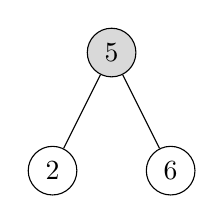
\begin{tikzpicture}
    \node[circle,draw,fill=gray!30](z){5}
        child {
          node[circle,draw]{2}
          child[missing]
          child[missing]
        }
        child{
          node[circle,draw]{6}
          child[missing]
          child[missing]
        };
  \end{tikzpicture}%
  \hspace{1cm}%
      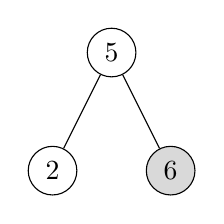
\begin{tikzpicture}
      \node[circle,draw](z){5}
        child {
          node[circle,draw]{2}
          child[missing]
          child[missing]
        }
        child{
          node[circle,draw,fill=gray!30]{6}
          child[missing]
          child[missing]
        };
    \end{tikzpicture}%
    \hspace{1cm}%
    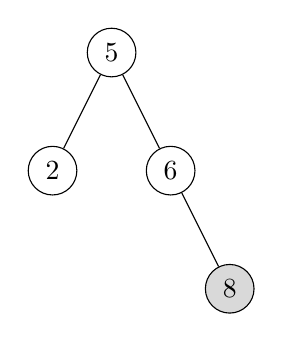
\begin{tikzpicture}
      \node[circle,draw](z){5}
        child {
          node[circle,draw]{2}
          child[missing]
          child[missing]
        }
        child{
          node[circle,draw]{6}
          child[missing]
          child {
            node[circle,draw,fill=gray!30]{8}
            child[missing]
            child[missing]
          }
        };
    \end{tikzpicture}
    \caption{Example of an insertion operation with key 8}
    \label{fig:insert}
\end{figure}

An AVL tree is based on a binary search tree, with one very important distinction - it is \textit{balanced}. To define what it means for a tree to be balanced, I will first
define what the \textit{height} of a tree is.

\begin{definition}[Tree height]
  \label{def:height}
  The height of a tree is the length of the longest path from the root to a leaf.
\end{definition} 
 
Balance is reliant on this definition - an AVL tree is only balanced when the 
heights of any given left and right child subtrees does not differ by more than one \cite{avl:original}. By keeping balance, the structure ensures that there is a high ratio between the number of 
nodes in the tree and the height. This allows for retrieval and search operations to be done in $O(\log n)$ time in the worst case, with $n$ being the amount of nodes in a tree \cite{avl:computer}. A
balancing factor can help define whether a tree is balanced or not.

\begin{definition}[Balancing factor]
  \label{def:bf}
  The balancing factor $BF(n)$ of a tree is the difference in height between the left child tree and the right child tree. A tree is defined to be an AVL tree (and therefore balanced) is the
  invariant $BF(n) \in \{-1,0,1\}$ holds for every node $n$ in the tree.
\end{definition}

During node insertion, the tree can become imbalanced, which can be mitigated
with either a right rotation or a left rotation. 

\begin{figure}[!ht]
  \centering
  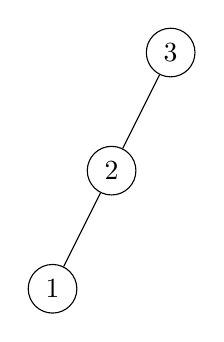
\begin{tikzpicture}
    \node[circle,draw](z){3}
      child {
        node[circle,draw]{2}
        child {
          node[circle,draw]{1}
          child[missing]
          child[missing]
        }
        child[missing]
      }
      child[missing];
  \end{tikzpicture}%
  \hspace{1cm}%
  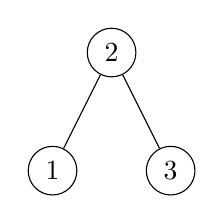
\begin{tikzpicture}
    \node[circle,draw](z){2}
    child{
      node[circle,draw]{1}
      child[missing]
      child[missing]
    }
    child{
      node[circle,draw]{3}
      child[missing]
      child[missing]
    };
  \end{tikzpicture}
  \caption{Example of a single right rotation}
  \label{fig:right_rotation}
\end{figure}